\chapter{Diseño e Implementación} % Main chapter title

\label{Chapter3} % Change X to a consecutive number; for referencing this chapter elsewhere, use \ref{ChapterX}
\definecolor{mygreen}{rgb}{0,0.6,0}
\definecolor{mygray}{rgb}{0.5,0.5,0.5}
\definecolor{mymauve}{rgb}{0.58,0,0.82}

\lstset{ %
  backgroundcolor=\color{white},   % choose the background color; you must add \usepackage{color} or \usepackage{xcolor}
  basicstyle=\footnotesize,        % the size of the fonts that are used for the code
  breakatwhitespace=false,         % sets if automatic breaks should only happen at whitespace
  breaklines=true,                 % sets automatic line breaking
  captionpos=b,                    % sets the caption-position to bottom
  commentstyle=\color{mygreen},    % comment style
  deletekeywords={...},            % if you want to delete keywords from the given language
  %escapeinside={\%*}{*)},          % if you want to add LaTeX within your code
  %extendedchars=true,              % lets you use non-ASCII characters; for 8-bits encodings only, does not work with UTF-8
  %frame=single,	                   % adds a frame around the code
  keepspaces=true,                 % keeps spaces in text, useful for keeping indentation of code (possibly needs columns=flexible)
  keywordstyle=\color{blue},       % keyword style
  language=[ANSI]C,					% the language of the code
  %otherkeywords={*,...},           % if you want to add more keywords to the set
  numbers=left,                    % where to put the line-numbers; possible values are (none, left, right)
  numbersep=5pt,                   % how far the line-numbers are from the code
  numberstyle=\tiny\color{mygray}, % the style that is used for the line-numbers
  rulecolor=\color{black},         % if not set, the frame-color may be changed on line-breaks within not-black text (e.g. comments (green here))
  showspaces=false,                % show spaces everywhere adding particular underscores; it overrides 'showstringspaces'
  showstringspaces=false,          % underline spaces within strings only
  showtabs=false,                  % show tabs within strings adding particular underscores
  stepnumber=1,                    % the step between two line-numbers. If it's 1, each line will be numbered
  stringstyle=\color{mymauve},     % string literal style
  tabsize=2,	                   % sets default tabsize to 2 spaces
  title=\lstname,                   % show the filename of files included with \lstinputlisting; also try caption instead of title
  morecomment=[s]{/*}{*/}%
}


%----------------------------------------------------------------------------------------
%	SECTION 1
%----------------------------------------------------------------------------------------
\section{Diseño e Implementación}
En este capítulo se verá como se desarroló un hardware básico para poder simular el entorno de funcionamiento y como fue implementado el firmware.
%La idea de esta sección es resaltar los problemas encontrados, los criterios utilizados y la justificación de las decisiones que se hayan tomado.
%Se puede agregar código o pseudocódigo dentro de un entorno lstlisting con el siguiente código:

\section{Hardware}

Se implemento el diseño de un circuito, el cual permitiria simular el entorno de funcionamiento de la bodega. Para ello se utilizó lo aprendido a la largo del curso de \emph{diseño de PCBs en KICAD}. El sistema cuanta con:
  \begin{itemize}
    \item 1 Salida con regulacion de corriente, para simular sensores de 4mA a 20mA. Figura \ref{fig:temp_tens}.
    \item 1 Salida con tension variable, utilizando el regulador LM317. Figura \ref{fig:temp_tens}.
    \item 1 Salida del sensor de temperatura LM35. Figura \ref{fig:temp_tens}.
    \item 2 Salidas con tensión variable, utilizando potenciometros. Figura \ref{fig:temp_tens}.
    \item 4 Entradas digitales conectadas a leds. Figura \ref{fig:pul_leds}.
    \item 4 Salidas conectadas a pulsadores. Figura \ref{fig:pul_leds}.
    \item 1 Socalo para la conxion del modulo SIM800L. Figura \ref{fig:essim800}.
    \item 1 salida de 5V a 3A y otra de 3.3V a 1A. Figura \ref{fig:fuente}.
  \end{itemize}

El esquemático implementado es el siguiente:
\begin{figure}[h]
      \centering
      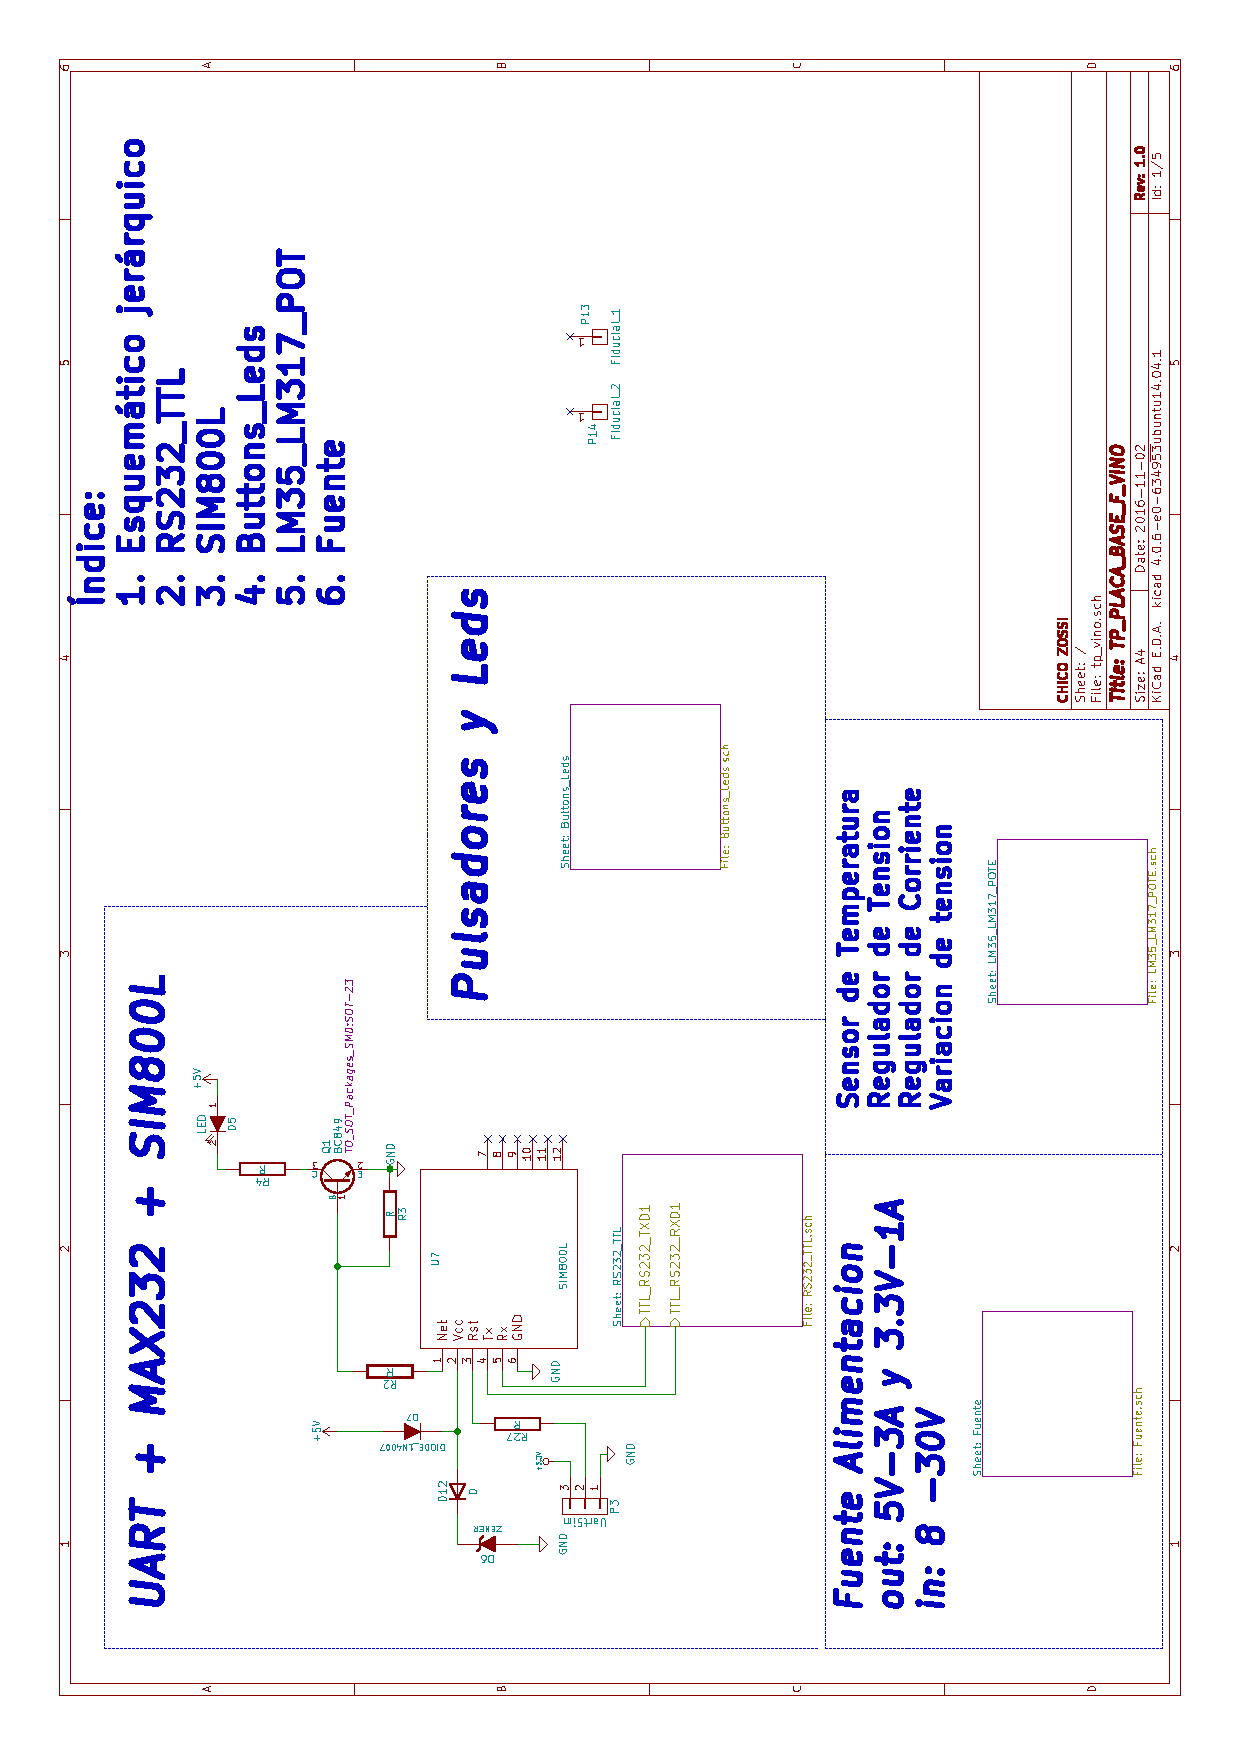
\includegraphics[page=1,scale=0.3,angle=270]{./Figures/schematic.pdf}
      \caption{Esquemático para la coneccion del módulo sim800l e indice de esquemáticos.}
      \label{fig:essim800}
\end{figure}

\begin{figure}[h]
      \centering
      \includegraphics[page=3,scale=0.3,angle=270]{./Figures/schematic.pdf}
      \caption{Esquemático de la fuente de alimentacion DC/DC.}
      \label{fig:fuente}
\end{figure}

\begin{figure}[h]
      \centering
      \includegraphics[page=4,scale=0.3,angle=270]{./Figures/schematic.pdf}
      \caption{Esquema del regulador de corriente, de tensión y del sensor de temperatura.}
      \label{fig:temp_tens}
\end{figure}

\begin{figure}[h]
      \centering
      \includegraphics[page=5,scale=0.3,angle=270]{./Figures/schematic.pdf}
      \caption{Esquema entradas a leds y salidas de los pulsadores.}
      \label{fig:pul_leds}
\end{figure}


El modulo sim800l que se muestra en la siguiente Figura \ref{fig:sim800l}, es un modem gprs que cuenta con las siguientes especificaciones:

\begin{figure}[h]
      \centering
      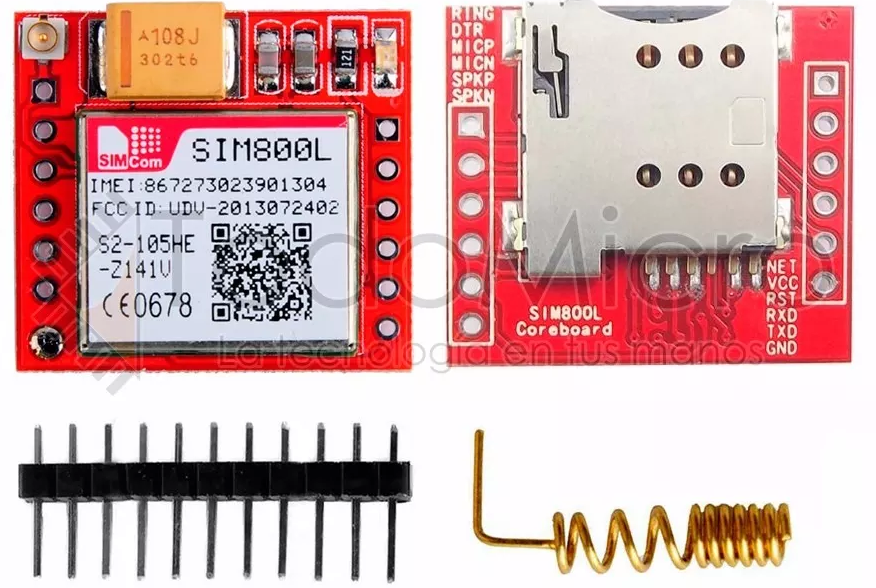
\includegraphics[scale=0.2]{./Figures/sim800.png}
      \caption{Modem SIM800L.}
      \label{fig:sim800l}
\end{figure}

\begin{itemize}
 \item Alimentacion: 3.4V a 4.4V (4.0V recomendado)
 \item  Todos los pines del módulo disponibles en pads de 2.54mm.
 \item  CuatriBanda 850/900/1800/1900MHz
 \item  GPRS Multi Slot class 8/10
 \item  Control mediante comandos AT (GSM 07.07 ,07.05 y comandos AT SIMCOM).
\end{itemize}

%
%\begin{verbatim}
%\begin{lstlisting}[caption= "un epígrafe descriptivo"]
%
%	las líneas de código irían aquí...
%	
%\end{lstlisting}
%\end{verbatim}
%
%A modo de ejemplo:
%
%\begin{lstlisting}[caption=Pseudocódigo del lazo principal de control.]  % Start your code-block
%
%#define MAX_SENSOR_NUMBER 3
%#define MAX_ALARM_NUMBER  6
%#define MAX_ACTUATOR_NUMBER 6
%
%uint32_t sensorValue[MAX_SENSOR_NUMBER];		
%FunctionalState alarmControl[MAX_ALARM_NUMBER];	//ENABLE or DISABLE
%state_t alarmState[MAX_ALARM_NUMBER];						//ON or OFF
%state_t actuatorState[MAX_ACTUATOR_NUMBER];			//ON or OFF
%
%void vControl() {
%
%	initGlobalVariables();
%	
%	period = 500 ms;
%		
%	while(1) {
%
%		ticks = xTaskGetTickCount();
%		
%		updateSensors();
%		
%		updateAlarms();
%		
%		controlActuators();
%		
%		vTaskDelayUntil(&ticks, period);
%	}
%}
%\end{lstlisting}
%


